\section{Постановка задачи}
Составьте блок-схему и напишите соответствующую ей программу, позволяющую
вычислять наибольший общий делитель двух больших натуральных чисел.


\clearpage
\section{Используемые инструменты}
Для решения вышеуказанной задачи были использованы следующие инструменты:
\begin{itemize}
    \item Основным ЯП был выбран Python версии 3.9.2;
    \item Для компиляции программы в бинарный файл .exe использован конвертер файлов Auto PY to EXE,
    который использует для своей работы PyInstaller.
\end{itemize}


\clearpage
\section{Общая структура библиотеки целых\\длинных чисел}
В библиотеке целых длинных содержится класс <<BigInt>>, рядом с которым объявлены следующие функции:
\begin{itemize}
    \item Реализации алгоритма Евклида для поиска НОД двух длинных целых чисел.\\
    Алгоритм был реализован для сравнения с более сложным алгоритмом того же назначения.
    \item Реализации бинарного алгоритма для поиска НОД двух длинных целых чисел.\\
    Данный алгоритм является более оптимальным, по сравнению с алгоритмом Евклида.
    Но в рамках использования языка Python он оказался более медленным, за счет частых преобразований
    строковых переменных в логические, для последующих операций битовых сдвигов.
\end{itemize}
Эти функции не являются методами класс <<BigInt>>, так как были реализованны таким образом,
что бы они могли работать как с экземплярами класса <<BigInt>>, так и с обычными переменным типа <<int>>.

Класс <<BigInt>> содержит в себе два основных поля:
\begin{enumerate}
    \item Поле хранения числа <<value>>.\\
    Представляет собой переменную типа строка, в котором содержится число экземпляра класса;
    \item Поле хранения знака числа <<is\_neg>>.\\
    Представляет собой переменную типа bool, в которой содержится информация о знаке числа.
    Значение True эквивалентно отрицательному числу, значение False - положительному;
\end{enumerate}

Создания экземпляра класса <<BigInt>> происходит следующие способами:
\begin{itemize}
    \item Создание экземпляра класса без передачи аргументов. Числовое значение такого экземпляра будет равно нулю.
    \begin{lstlisting}
a = BigInt()\end{lstlisting}
    \item Создание экземпляра класса с передачей в аргумент строки, которая может валидно быть приведена к типу целого числа.
    \begin{lstlisting}
a = BigInt('-1234567890')  # a = -1234567890
b = BigInt('1234567890')   # b = 1234567890
d = BigInt('0')            # d = 0\end{lstlisting}
    \item Создание экземпляра класса с передачей в аргумент целого числа.
    \begin{lstlisting}
a = BigInt(-1234567890)  # a = -1234567890
b = BigInt(1234567890)   # b = 1234567890
d = BigInt(0)            # d = 0\end{lstlisting}
    \item Создание экземпляра класса с передачей в аргумент экземпляра класса <<BigInt>>.
    \begin{lstlisting}
a = BigInt(-1234567890)  # a = -1234567890
b = BigInt(a)            # b = -1234567890\end{lstlisting}
\end{itemize}


\clearpage
\section{Примеры работы библиотеки}
В качестве примера работы будут использоваться прямые вызовы методов класса <<BigInt>>.

Пусть даны два целых длинных числа $a$ и $b$, сохраненных в экземпляр класса <<BigInt>>.
А так же, создадим экземпляр класса <<BigInt>> с нулевым значением.
    \begin{lstlisting}
a = BigInt('-1234567890987654321')
b = BigInt('9876543210123456789')
zero = BigInt()\end{lstlisting}

    \begin{itemize}
        \item Выполняем нахождение НОД двух длинных целых чисел с помощью алгоритма Евклида:
        \begin{lstlisting}
print(GDC(a, b))\end{lstlisting}
        Вывод: $9$
        \item Выполняем нахождение НОД двух длинных целых чисел с бинарного алгоритма:
        \begin{lstlisting}
print(binary_GCD(a, b))\end{lstlisting}
        Вывод: $9$
    \end{itemize}

\clearpage
\section{Вывод}
Мною был составлен алгоритм (в виде блок-схемы) и написана на языке Python программа, позволяющая:
\begin{itemize}
    \item вычислять наибольший общий делитель двух больших натуральных чисел с помощью алгоритма Евклида;
    \item вычислять наибольший общий делитель двух больших натуральных чисел с помощью бинарного алгоритма.
\end{itemize}

\clearpage
\section{Блок-схема методов библиотеки}
Ниже представлены блок-схемы функций в следующем порядке:
\begin{enumerate}
    \item Функция вычисления наибольшего общего делителя двух больших натуральных чисел с помощью алгоритма Евклида;
    \item Функция вычисления наибольшего общего делителя двух больших натуральных чисел с помощью бинарного алгоритма.
\end{enumerate}
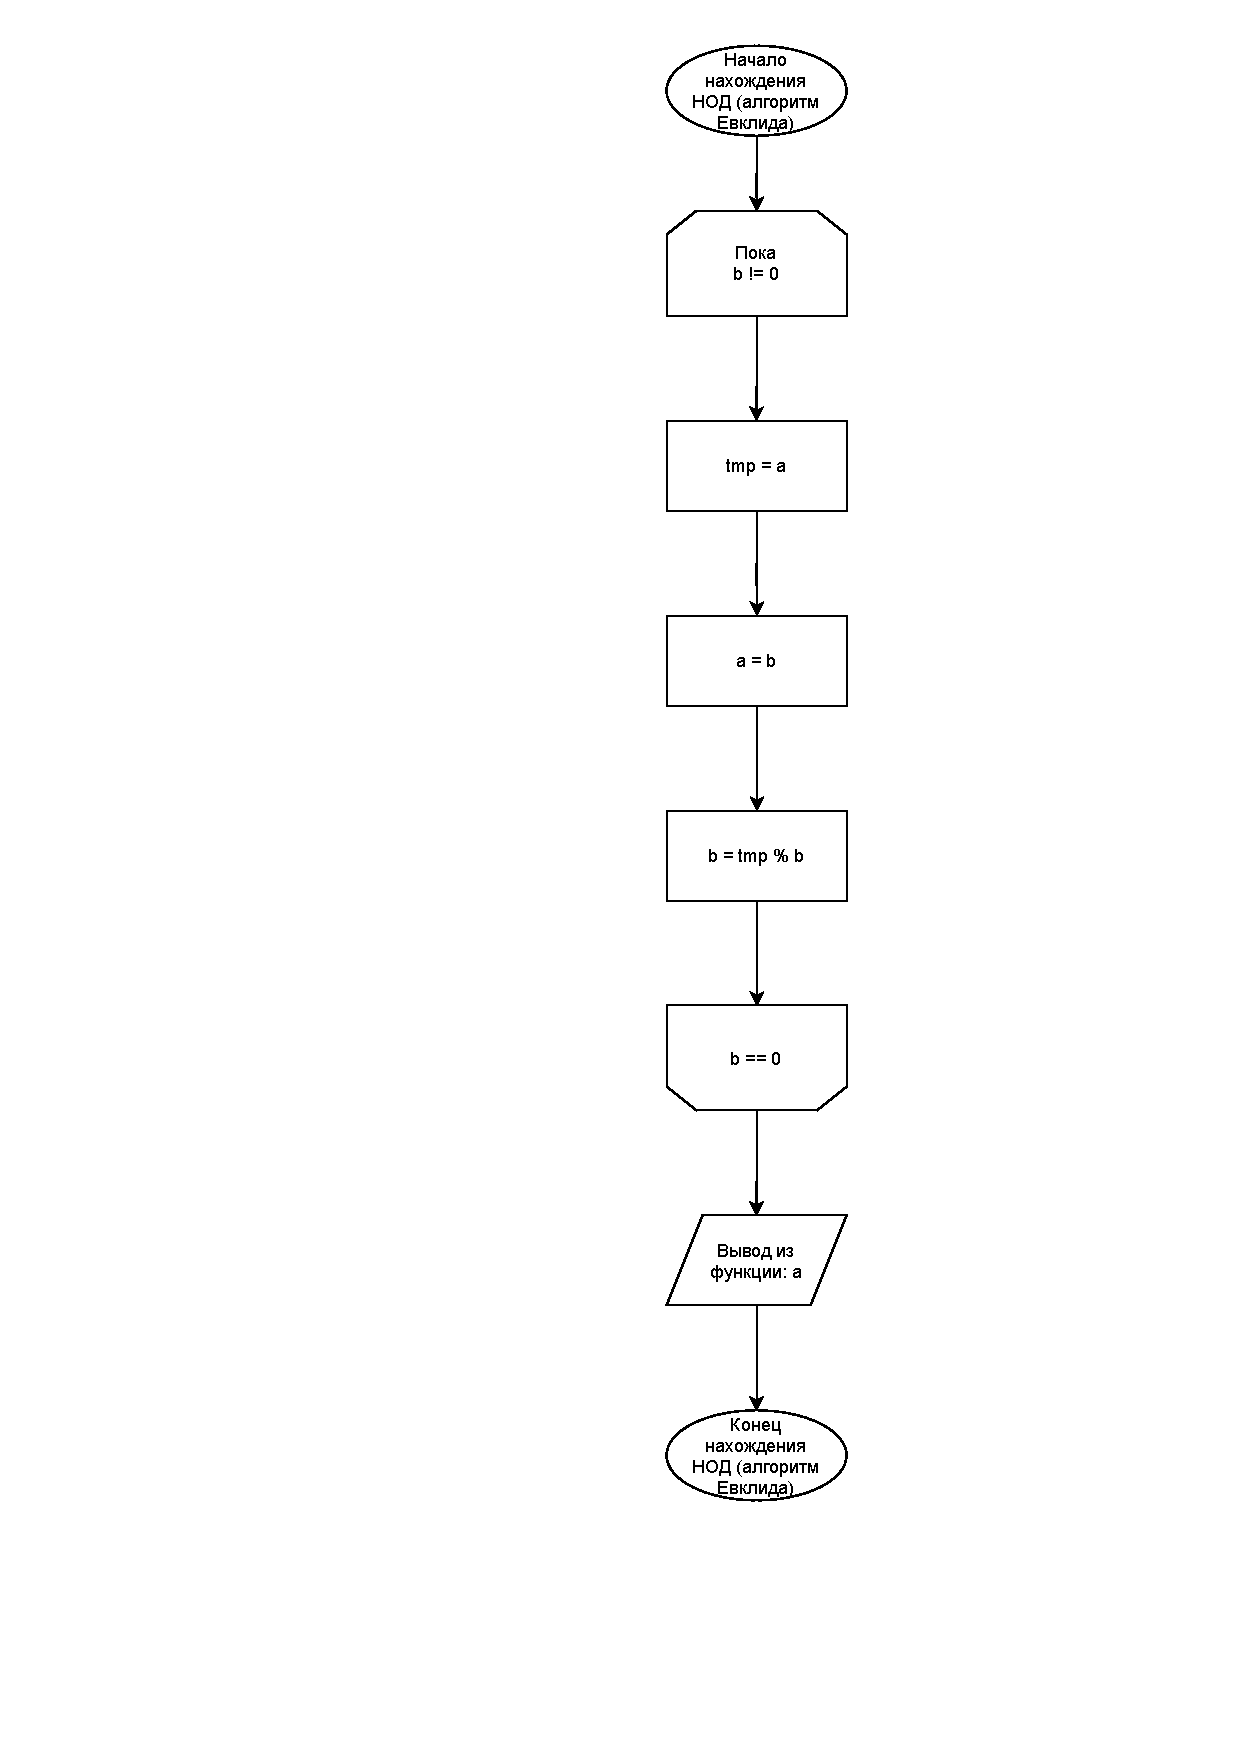
\includepdf[pages=-]{./Flowchart.pdf}
